\onehalfspacing
\section{Đề số 35}

\begin{bt} 
	\hfill
	\begin{enumerate}[1.]
		\item Tính giá trị của biểu thức
		$$
		\begin{aligned}
			& \mathrm{A}=(-1)^3 \cdot\left(-\frac{7}{8}\right)^3 \cdot\left(-\frac{2}{7}\right)^2 \cdot(-7) \cdot\left(-\frac{1}{14}\right) \\[5px]
			& \mathrm{B}=2016:\left(\frac{0,4-\frac{2}{9}+\frac{2}{11}}{1,4-\frac{7}{9}+\frac{7}{11}} \cdot \frac{-1 \frac{1}{6}+0,875-0,7}{\frac{1}{3}-0,25+\frac{1}{5}}\right)
		\end{aligned}
		$$
		\item Cho đa thức $Q(x)=a x^3+b x^2+c x+d$ với $a, b, c, d \in Z$. Biết $Q(x)$ chia hết cho 3 với mọi $x \in Z$. Chứng tỏ các hệ số $a, b, c, d$ đều chia hết cho 3.
	\end{enumerate}
	\loigiai{
		\begin{enumerate}
			\item $A=(-1) \cdot \frac{(-7)^3}{8^3} \cdot \frac{(-2)^2}{7^2} \cdot \frac{1}{2} \\[5px]
			= \frac{(-1) \cdot(-7)^3 \cdot(-2)^2}{2^9 \cdot 7^2 \cdot 2} \\[5px]
			= \frac{(-1) \cdot(-7) \cdot(-1)}{2^8} \\[5px]
			= \frac{-7}{256}$\\[5px]
			Tính:\\[5px]
			*) $ \frac{0,4-\frac{2}{9}+\frac{2}{11}}{1,4-\frac{7}{9}+\frac{7}{11}}=\frac{2 \cdot\left(\frac{1}{5}-\frac{1}{9}+\frac{1}{11}\right)}{7 \cdot\left(\frac{1}{5}-\frac{1}{9}+\frac{1}{11}\right)} \\[5px]
			= \frac{2}{7}\left(\text { vì } \frac{1}{5}-\frac{1}{9}+\frac{1}{11} \neq 0\right)$\\[5px] 
			*) $\frac{-1 \frac{1}{6}+0,875-0,7}{\frac{1}{3}-0,25+\frac{1}{5}}=\frac{-7 \cdot\left(\frac{1}{6}-\frac{1}{8}+\frac{1}{10}\right)}{2 \cdot\left(\frac{1}{6}-\frac{1}{8}+\frac{1}{10}\right)} \\[5px]
			=\frac{-7}{2}\left(\text { vì } \frac{1}{6}-\frac{1}{8}+\frac{1}{10} \neq 0\right) \\[5px]
			\text {B } = 2016:\left(\frac{2}{7} \cdot \frac{-7}{2}\right)=-2016$
			\item Cho đa thức $Q(x)=a x^3+b x^2+c x+d$\\[5px] $\text{Vì } \mathrm{Q}(\mathrm{x})$ : 3 với mọi $x \in Z$, nên\\[5px]
			$\text {Với } \mathrm{x}=0 \text {, ta có } \mathrm{Q}(0)=d \vdots 3 \\[5px]
			\text {Với } \mathrm{x}=1 \text {, ta có } \mathrm{Q}(1)=a+b+c+d \vdots 3 \\[5px]
			\text {mà } \mathrm{d} \vdots 3=>\mathrm{a}+\mathrm{b}+\mathrm{c} \vdots 3(1) \\[5px]
			\text {Với } \mathrm{x}=-1 \text {, ta có } \mathrm{Q}(-1)=-\mathrm{a}+\mathrm{b}-\mathrm{c}+\mathrm{d} \vdots 3 \\[5px]
			\text {mà } \mathrm{d} \vdots 3=>-\mathrm{a}+\mathrm{b}-\mathrm{c} \vdots 3(2) \\[5px]
			\mathrm{Q}(1)+\mathrm{Q}(-1)=2 \mathrm{~b} \vdots 3 \text { mà }(2 ; 3)=1 \text { nên } \mathrm{b} \vdots 3 \\[5px]
			\mathrm{Q}(1)-\mathrm{Q}(-1)=2(a+c) \vdots 3 \text { mà }(2 ; 3)=1 \text { nên } \mathrm{a}+\mathrm{c} \vdots 3(3) \\[5px]
			\text {Với } \mathrm{x}=2, \text { ta có } \mathrm{Q}(2)=8 \mathrm{a}+4 \mathrm{~b}+2 \mathrm{c}+\mathrm{d} \vdots 3 \\[5px]
			\text {hay } 7 \mathrm{a}+(\mathrm{a}+\mathrm{c})+2 \mathrm{~b}+\mathrm{d} \vdots 3 \\[5px]
			\text {Mà } \mathrm{d} \vdots 3, \mathrm{a}+\mathrm{c} \vdots 3, \mathrm{~b} \vdots 3 \text{ nên } 7 \mathrm{a} \vdots 3 \text { mà }(7 ; 3)=1=\mathrm{a} \vdots 3 \\[5px]
			\text {Từ (3) suy ra } \mathrm{c} \vdots 3=>\text{đpcm}$
		\end{enumerate}
	} 
\end{bt}

\begin{bt}
	\hfill
	\begin{enumerate}[1.]
		\item Biết $\frac{b z-c y}{a}=\frac{c x-a z}{b}=\frac{a y-b x}{c}($ với $a, b, c \neq 0)$.
		Chứng minh rằng: $\frac{\mathrm{x}}{\mathrm{a}}=\frac{\mathrm{y}}{\mathrm{b}}=\frac{\mathrm{z}}{\mathrm{c}}$.
		\item Số $\mathrm{M}$ được chia thành ba phân tỉ lệ nghịch với $3 ; 5 ; 6$. Biết rằng tổng các lập phương của ba phần đó là 10728 . Hãy tìm số $\mathrm{M}$.
	\end{enumerate}
	\loigiai{
		\begin{enumerate}
			\item Với a, b, c $\neq 0$, ta có:\\[5px]
			$\frac{b z-c y}{a}=\frac{c x-a z}{b}=\frac{a y-b x}{c}=\frac{b z a-c y a}{a^2}=\frac{b c x-b a z}{b^2}=\frac{a c y-b c x}{c^2} \\[5px]
			=\frac{b z a-c y a+b c x-b a z+a c y-b c x}{a^2+b^2+c^2}=\frac{0}{a^2+b^2+c^2}=0$\\[5px]
			Suy ra $\frac{\mathrm{bz}-\mathrm{cy}}{\mathrm{a}}=0$, do đó $\mathrm{bz}=\mathrm{cy} \Rightarrow \frac{\mathrm{y}}{\mathrm{b}}=\frac{\mathrm{z}}{\mathrm{c}}(1)$\\[5px]
			$\frac{\mathrm{cx}-\mathrm{az}}{\mathrm{b}}=0, \text { do đó } \mathrm{cx}=\mathrm{az} \Rightarrow \frac{\mathrm{x}}{\mathrm{a}}=\frac{\mathrm{z}}{\mathrm{c}}$ (2)\\[5px]
			Từ (1) và (2) suy ra $\frac{\mathrm{x}}{\mathrm{a}}=\frac{\mathrm{y}}{\mathrm{b}}=\frac{\mathrm{c}}{\mathrm{z}}$
			\item Gọi ba phần được chia của số $M$ là $x, y, z$. , ta được $x+y+z=M$\\[5px]
			Theo đề bài ta có $\mathrm{x}: \mathrm{y}: \mathrm{z}=\frac{1}{3}: \frac{1}{5}: \frac{1}{6}$ và $x^3+y^3+z^3=10728(1)$\\[5px]
			Hay $\frac{\mathrm{x}}{10}=\frac{\mathrm{y}}{6}=\frac{\mathrm{z}}{5}=k$ và $x^3+y^3+z^3=10728$\\[5px]
			Suy ra $x^3=10^3 \cdot k^3 ; y^3=6^3 \cdot k^3 ; z=5^3 \cdot k^3$\\[5px]
			Thay vào (1), được $1341 k^3=8 \Rightarrow k=2$
			suy ra $20 ; y=12 ; z=10 \quad$\\[5px] 
			Vậy $M=42$.
		\end{enumerate}
	} 
\end{bt}

\begin{bt}
	Cho tam giác $\mathrm{ABC}$ đều. Trên cạnh $\mathrm{AB}$ lấy điểm $\mathrm{D}$ sao cho $\mathrm{BD}=\frac{1}{3} \mathrm{AB}$. Tại $\mathrm{D}$ kẻ đường vuông góc với $\mathrm{AB}$ cắt cạnh $\mathrm{BC}$ tại $\mathrm{E}$. Tại $\mathrm{E}$ kẻ đường vuông góc với $\mathrm{BC}$ cắt $\mathrm{AC}$ tại $\mathrm{F}$.
	\begin{enumerate}[1.]
		\item Chứng minh $\mathrm{DF} \perp \mathrm{AC}$. Biết trong tam giác vuông cạnh đối diện với góc $30^{\circ}$ thì bằng nửa cạnh huyền.
		\item Chứng minh tam giác DEF đều.
		\item Gọi $G$ là trọng tâm của tam giác $D E F$. Chứng minh $G A=G B=G C$.
	\end{enumerate}
	\loigiai{
		$$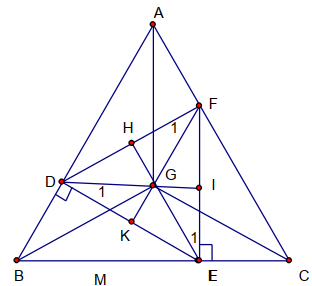
\includegraphics[width=0.45\textwidth]{35-3-lg.png}$$
		\begin{enumerate}
			\item $\triangle \mathrm{ABC}$ đều nên $\mathrm{AB}=\mathrm{AC}=\mathrm{BC}=\mathrm{a}$ và $\angle \mathrm{A}=\angle \mathrm{B}=\angle \mathrm{C}=60^{\circ}$\\[5px]
			$\mathrm{BD}=\frac{1}{3} \mathrm{a} \quad$ (gt)\\[5px] $\Rightarrow \mathrm{AD}=\frac{2}{3} \mathrm{a}$\\[5px]
			Xét $\triangle \mathrm{BDE}$ vuông tại $\mathrm{D}$ có $\angle \mathrm{B}=60^{\circ} \Rightarrow \angle \mathrm{DEB}=30^{\circ}$\\[5px]
			Xét $\triangle \mathrm{BDE}$ vuông tại $\mathrm{D}$ có $\angle \mathrm{DEB}=30^{\circ}\\[5px] 
			\Rightarrow \mathrm{BD}=\frac{1}{2} \mathrm{BE}$\\[5px]
			hay $\mathrm{BE}=2 \mathrm{BD}=2 \cdot \frac{1}{3} \mathrm{a}=\frac{2}{3} \mathrm{a}$ mà $\mathrm{BC}=\mathrm{a}$ nên $\mathrm{EC}=\frac{1}{3} \mathrm{a}$\\[5px]
			Tương tự, xét $\triangle \mathrm{ECF}$ vuông tại $\mathrm{E}$ có $\angle \mathrm{C}=60^{\circ}\\[5px] \Rightarrow \angle \mathrm{EFC}=30^{\circ}$\\[5px]
			$\Rightarrow \mathrm{AF}=\frac{1}{3} \mathrm{a}$\\[5px]
			Xét $\triangle \mathrm{ADF}$ và $\triangle \mathrm{BED}$ có:\\[5px]
			$\mathrm{AD}=\mathrm{BE}\left(=\frac{2}{3} \mathrm{a}\right)$\\[5px]
			$\angle \mathrm{A}=\angle \mathrm{B}\left(=60^{\circ}\right)$\\[5px]
			$\mathrm{AF}=\mathrm{BD}\left(=\frac{1}{3} \mathrm{a}\right)$\\[5px]
			$\Rightarrow \triangle \mathrm{ADF}=\triangle \mathrm{BED}($ c. g. c)\\[5px]
			$\Rightarrow \angle \mathrm{AFD}=\angle \mathrm{BDE}$ ( hai góc tương ứng)\\[5px]
			Mà $\angle \mathrm{BDE}=90^{\circ} \\[5px]
			\Rightarrow \angle \mathrm{AFD}=90^{\circ}$ hay $\mathrm{DF} \perp \mathrm{AC}$
			\item Chứng minh tương tự cũng có $. \Delta \mathrm{DBE}=\Delta \mathrm{ECF}$ (c.g.c)\\[5px] 
			$\Rightarrow \mathrm{DE}=\mathrm{EF}$ ( hai cạnh tương ứng)\\[5px] 
			Có $\triangle \mathrm{ADF}=\Delta \mathrm{BED}$ ( c. g. $\mathrm{c}$ ) $(\mathrm{cmt})\\[5px] 
			\Rightarrow \mathrm{DF}=\mathrm{DE}$ ( hai cạnh tương ứng)\\[5px] 
			$\Rightarrow \mathrm{DE}=\mathrm{DF}=\mathrm{EF}\\[5px] \Rightarrow \Delta \mathrm{DEF}$ là tam giác đều.
			\item Xét $\triangle D E F$ đều có $G$ là trọng tâm của tam giác\\[5px] 
			$\Rightarrow G$ là giao điểm của ba đường phân giác\\[5px] 
			$\Rightarrow \mathrm{GD}, \mathrm{GE}, \mathrm{GF}$ là các đường phân giác của các góc $\angle \mathrm{EDF} ; \angle \mathrm{DEF} ; \angle \mathrm{DFE}$ Có $\triangle \mathrm{DEF}$ đều nên $\angle \mathrm{D}=\angle \mathrm{E}=\angle \mathrm{F}=60^{\circ}$
		\end{enumerate}
	}
\end{bt}

\begin{bt}
	Cho tam giác $\mathrm{ABC}$, trung tuyến $\mathrm{AM}$ và $\mathrm{BE}$ cắt nhau tại $\mathrm{G}$. Chứng minh rằng nếu $\mathrm{AGB} \leq 90^{\circ}$ thì $\mathrm{AC}+\mathrm{BC}>3 \mathrm{AB}$.
	\loigiai{
		$$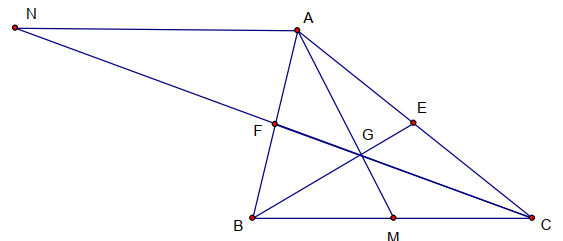
\includegraphics[width=0.65\textwidth]{35-4-lg.png}$$
		Vẽ trung tuyến CF của Tam giác $\mathrm{ABC}$. Trên tia đối của tia $F C$ lấy điểm $\mathrm{N}$ sao cho $\mathrm{FN}=\mathrm{FC}$.\\[5px]
		$\mathrm{C} / \mathrm{M}$ được $: \triangle \mathrm{ANF}=\Delta \mathrm{BCF}(\mathrm{c}-\mathrm{g}-\mathrm{c}) \Rightarrow \mathrm{AN}=\mathrm{BC}$\\[5px]
		Xét $\triangle \mathrm{CAN}$ có $\mathrm{AN}+\mathrm{AC}>\mathrm{NC}$ ( bất đẳng thức tam giác)\\[5px]
		$\Rightarrow \mathrm{AC}+\mathrm{BC}>\mathrm{NC}$\\[5px]
		Vì $\mathrm{G}$ là trọng tâm của tam giác $\mathrm{ABC}$ nên $\mathrm{CF}=3 \mathrm{GF} \Rightarrow \mathrm{NC}=6 \mathrm{GF}$ (1)\\[5px]
		Ta sẽ chứng minh: nếu $\angle \mathrm{AGB} \leq 90^{\circ}$ thì $\mathrm{GF} \geq \frac{A B}{2}$\\[5px]
		Giả sử $\mathrm{GF}<\frac{A B}{2}$ hay $\mathrm{GF}<\mathrm{AF}=\mathrm{BF}$ thì $\angle \mathrm{FAG}<\angle \mathrm{AGF} ; \angle \mathrm{FBG}<\angle \mathrm{BGF}$ ( quan hệ góc và cạnh tương ứng trong tam giác)\\[5px]
		$\Rightarrow \angle \mathrm{ABG}+\angle \mathrm{BAG}<\angle \mathrm{FGB}+\angle \mathrm{FGA}=\angle \mathrm{AGB} \leq 90^{\circ}$\\[5px]
		Xét tam giác $\mathrm{AGB}$ có $\angle \mathrm{ABG}+\angle \mathrm{BAG}+\angle \mathrm{AGB}<90^{\circ}+90^{\circ}=180^{\circ}$ vô lí.\\[5px]
		Vậy nếu $\angle \mathrm{AGB} \leq 90^{\circ}$ thì $\mathrm{GF} \geq \frac{A B}{2}$ (2)\\[5px] 
		$\text { Từ (1) và (2) } \Rightarrow N C \geq 3 A B \text { suy ra } \mathrm{AC}+\mathrm{BC}>3 \mathrm{AB} \text { (đpcm) }$
	} 
\end{bt}

\begin{bt}
	Tìm các giá trị nguyên của $x$ để biểu thức $C=\frac{22-3 x}{4-x}$ có giá trị lớn nhất.
	\loigiai{
		Biến đổi $C=\frac{22-3 x}{4-x}=\frac{3(4-x)+10}{4-x}=3+\frac{10}{4-x}$\\[5px]
		C có giá trị lớn nhất khi và chỉ khi $\frac{10}{4-x}$ có giá trị lớn nhất\\[5px]
		Có $x \in Z$, ta xét các trường hợp sau:\\[5px]
		Với $x>4 \Rightarrow 4-x<0$ thì $\frac{10}{4-x}<0$\\[5px]
		Với $x>4 \Rightarrow 4-x>0$.\\[5px] 
		Phân số $\frac{10}{4-x}$ có tử và mẫu đều dương, tử không đổi nên có giá trị lớn nhất khi mẫu nhỏ nhất\\[5px]
		Có $x \in Z$ Suy ra $4-x \in Z$\\[5px]
		Suy ra $4-x$ là số nguyên dương nhỏ nhất $\Rightarrow 4-x=1 \Rightarrow x=3$\\[5px]
		khi đó $\frac{10}{4-x}$ có giá trị là $10(2)$\\[5px]
		Từ (1) và (2) , phân số $\frac{10}{4-x}$ lớn nhất bằng 10\\[5px]
		Vậy GTLN của $C$ bằng 13 khi và chỉ khi $x=3$
	}
\end{bt}
